\chapter{Úvod}

%\section{Úvod a motivácia}
Žvasty o tom koľko je útokov zbrani v ČR a pod...


% ------------ NEW CHAPTER ------------
\chapter{Technológie}

V tejto kapitole sa zoznámime so základnymi pojmami a princípmi, ktoré súvia s probletikou tejto práce a ktoré budú dalej využívané.
Kapitola vysvetľuje základne rozdelenia zbraní, princíp spracovania digitálneho obrazu a metódy jeho predspracovanie.
Ďalej sú tu vysvetlené rôzne spôsoby pre klasifikáciu týchto obrazových dát.

% http://scikit-learn.org/stable/tutorial/machine\_learning\_map/index.html
% 16008.pdf - Klasifikacne algoritmy - str.10+
% imagenet-classification-with-deep-convolutional-neural-networks.pdf - Introduction str.1+
% Rozpoznávání-termosnímků-obličeju.pdf
% 9614.pdf

\section{Zbrane}
Obvýklá definícia hovorí, že zbraň je nástroj, predmet, či dokonca celé zariadenie,
ktoré je prispôsobené k vyvolaniu ranivého účinku na živý organizmus alebo k ničeniu objektu\cite{book:StrelneZbrane}.
Za prvé zbrane môžeme považovať kopije ktoré používali luďia pri love zvierat asi pred 400,000 rokmi\cite{prop:SpearHistory}.

Vo všeobecnosti môžeme zbrane rozdeliť podľa množstvá krytérií, napr. podľa zdroja energie použitej k vypudeniu projektilu zo zbrane,
podľa konštrukcie a režimu streľby, ďalej z hľadiska postupu pri nabíjaní alebo podľa veku zbrane na nové - slúžiace svojmu účelu a historické - ktoré sú uź nespôsobilé k pôvodnemu účelu.
My sa zameriame na 2 základne rozdelenia a to poďla toho ako zbrane pôsobia na živú sílu[cz. živou sílu], delíme na\cite{book:StrelneZbrane}:
\begin{enumerate}
	\item[$\bullet$] \textbf{Strelné} - rozrušujú vzdialený cieľ, živý alebo neživý, prodstredníctvom depadovej energie strely vypudenej zo zbrane.
	\item[$\bullet$] \textbf{Chladné} - účinkujú bodom alebo sekom naostrenej čepele, ktorá je vsadená do rukoväťe lebo je nasadená na tyč alebo porísko.
    \item[$\bullet$] \textbf{Úderné} - pôsobia na živý objekt tupým úderom s vojej časti, tkorá býva spojená s vhodnou rukoväťou.
\end{enumerate}
a podľa ovládateľnosti a možnosti prenášania ich delíme na\cite{book:StrelneZbrane}:
\begin{enumerate}
	\item[$\bullet$] \textbf{Ručné} strelné zbrane môže prenášať a ovládať jediná osoba. Sú ovládané buď jednou rukou - krátke zbrane - alebo oboma rukami - dlhé zbrane.
	\item[$\bullet$] \textbf{Lafetované} zbrane musia byť vzhľadom ku svojej hmotnosti a rozmerom umiestnené na zvláštnom podstavci - \textit{lafete}. Takúto zbraň takisto väčsinou obsluhuje viac ľudí.
\end{enumerate}
V tejto práci sa zameramé hlavne na strelné, ručné zbrane.

\section{Spracovanie obrazu}
Pre popis obrázkov a ostatných signálov sú často používané matematické modely.
Kde signál je funkcia závislá na nejakých premenných s fyzikálnym významom, môže byť 1-dimenzionálna (napr. závisla na čase),
2-dimenzionálna (napr. obrázok závislý na 2 koordinátoch v ploche), 3-dimenzionálna (napr. popis pozície objektu v priestore), alebo aj viac-dimenzionálna\cite{book:ImageProcessing}.

    Každý obraz môže byť definovaný ako spojitá funkcia s dvomi neznámymi $$f(x,y)$$ kde $x$ a $y$ sú súradnice v ploche.
Tento spojitý obraz je digitalizovaný na tzv. vzorkovacích miestach.
Tieto vzorkovacie miesta sú usporiadané v ploche, ich geometrický vzťah sa nazýva mriežka.
Digitálny obraz je potom dátova štruktúra, ktorá je bežne reprezentovaná ako matica.
Jeden bod v mriežke reprezentuje jeden element 2-dimenzionálneho obraze nazývany pixel, v 3-dimenzionálnom obraze sá tento element nazýva voxel\cite{book:ImageProcessing}.
Pri viac-dimenzionálnych digitálnych obrazoch sa pri spracovaní obrazu používa vektor hodnôt(napr. RGB hodnoty obrazového bodu).

Oblasť spracovania digitálneho obrazu je v dnešnej dobe veľmi široká a nachádza uplatnenie vo viacerých oboroch.
Môže sa využívať pri automatickej vizuálnej inšpekcií produktou, pre zaistenie vyššej produktivity a kvality výrobku v továrňach.
Ďalej pri spracovaní snímkou z lietadiel alebo satelitou pre získanie dát o prírodnych zdrojoch, ako napr. v poľnohospodárstve alebo lesníctve.
Širokú aplikáciu má v medicíne pri obrázkoch získavaných pomocou röngenových zariadení, CT a magnetickej rezonancie\cite{book:ImageProcessingApplication}.
A v súčastnosti v automobilovom priemysle pri rozvýjajúcej sa oblati autonómneho riadenia automobilov.

\section{Klasifikácia}

\# TODO - dopisať čo je to Klasifikácia

\subsection{K-Nearest-Neighbor}
\textit{k}-Nearest Neighbor je algoritmus ktorý sa učí pod dozorom [eng. supervised learning algorithm] často používaný pri rozpoznávaní vzorov v klasifikácií,
avšak je možné ho použiť aj pre odhad a predikciu\cite{book:DataMining}.
Algoritmus je pamäťovo náročný [eng. memory-based] a nepotrebuje žiaden model.
Pre jeho fungovanie nie je potrebný žiaden explicitný postup trénovania, okrem zberu vektorov príznakov s označeniami tried do ktorých patria.

Klasifikácia dát prebieha v 2 krokoch: nájdenie \textit{k} najbližších susedov spomedzi trénovaných dát a
vykonanie "väčšinové hlasovanie" medzi nájdenými susedmi pre priradenie najčastejšie sa vykytovaného označenia triedy.

Nech $\{ (x_i, y_i), i = 1, 2, \dots, n \}$ je množína trénovacích dát, kde $x_i$ je vektor príznakov a $y_i$ je názov triedy do ktorej patrí vektor $x_i$.
Predpokladáme že každé $x_i$ je v nejakom multidimenzionálnom priestore príznakov s metrikov $P$ a $y_i \in \{ 1, 2, \dots, l \}$, kde $l$ je číslo odpovedajúcej triedy.
Cieľom je priradiť neoznačeny vektor $x$ do zodpovedajucej triedy z množiny $\{ 1, 2, \dots, l \}$.

Najjednoduchšia verzia algoritmu \textit{k}-NN je 1-NN, kde vektor $x$ je priradený najbližsiemu susedovy.
To znamená že ak $x_j$, kde $j \in \{ 1, 2, \dots, n \}$, je najbližšií k $x$ vo forme vzdialenosti $P$ \cite{prop:KnnClassification}:
\begin{equation}
    \label{eq:kNNMetric}
    x_j = arg \; min_{\{x_i, 1 \leq i \leq n\}} P(x, x_i)
\end{equation}
tak označenie triedy pre vektor $x$ je číslo $y_i$.

Pre formu algoritmu \textit{k}-NN, kde $k > 1$ je postup podobný, ale priradenie označenia triedy pre $x$ je na základe najčastejšie sa vyskutovaného označenia triedy
spomedzi \textit{k} najbližších susedov z trénovacých bodov $x_i$, kde $k$ je užívateľom definovaná konštanta \cite{prop:KnnClassification}.

Najbežnejší výpočet pre vzdielenosť bodov je pomocou Euklidovskej vzdielenosti.
Táto vzdielnosť je medzi dvoma $J$-dimenzionálnymi vektormi $a$ a $b$ vyjadrená ako \cite{prop:KnnClassification}:
\begin{equation}
    \label{eq:euclidMetric}
    d_{a,b} = \sqrt{\sum_{j=1}^{J}{(a_j - b_j)^2}}
\end{equation}

Na obrázku \ref{pic:kNN} je zobrazený rozdiel medzi 1-NN a 5-NN algoritmom pre klasifikáciou,
    použitím 2-dimenzionálnych bodov a 3 tried dát (červená, modrá, zelená).
Farebné regióny vyznačujú rozhodovacie hranice klasifikátora, ktorý využíva Euklidovskú vzdielnosť.
Biele oblasti ukazujú body, ktoré sú nejednoznačne klasifikované (to znamená, že hodnotenie triedy je viazané aspoň na dve triedy).
V ukážke je vidno že v prípade 1-NN klasifikátora, niektré body vytvárajú "malé ostrovy"
    (napr. zelený bod v strede mraku medzi modrými bodmi), zatiaľ čo 5-NN klasifikátor vyhladzuje tieto nezrovnalosti,
    a pravdepodobne vedie k lepšiemu zovšeobecneniu nad testovacími údajmi.

\begin{figure}[H]
	\centering
	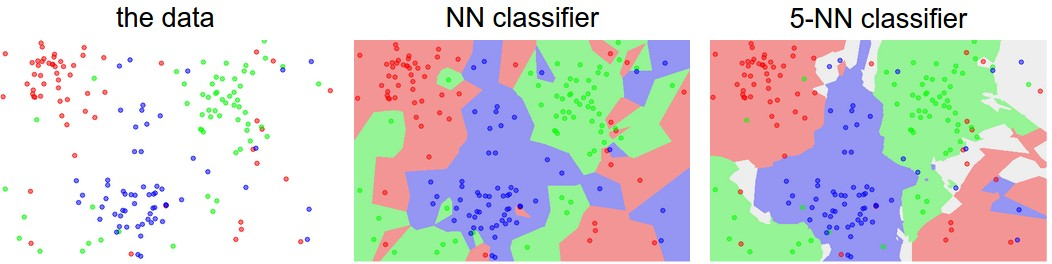
\includegraphics[width=1\textwidth]{knn}
	\caption{Porovnanie k-NN klasifikátorov\cite{odkaz:KnnImage}}
	\label{pic:kNN}
\end{figure}

\subsection{Support Vector Machines}

Support Vector Machines (SVM's) sú metódy učenia používané pre binárnu klasifikáciu.
Základnou myšlienkou je nájdenie hyper--roviny ktorá perfektne oddelí \textit{d}--dimenzionálne dáta do dvoch tried\cite{prop:IntroductionToSVM}.
SVM sa snaží maximalizovať vzdialenosť medzi rozdeľujúcov rovinou a dátami nachádzajúcimi sa v každej z 2 polrovín\cite{prop:SupervisedMachineLearning}.
Avšak kedže vstupné dáta väčšinou niesu lineárne separovatelné, SVM's predstavujú pojem "jadrový priestor indukovaný príznakom"[eng. “kernel induced feature space”],
    ktorý prevádza dáta do vyššieho dimenzionálneho pristoru, kde dáta sú oddeliteľné.\cite{prop:IntroductionToSVM}

Ak trénovacie dáta sú lineárne separovatelné, tak dvojica $(w, b)$ existuje ako\cite{prop:SupervisedMachineLearning}:
\begin{equation}
    \label{eq:SVMPair1}
    w^T * x_i + b \geq 1, \; pre \; x_i \in P
\end{equation}
\begin{equation}
    \label{eq:SVMPair2}
    w^T * x_i + b \leq -1, \; pre \; x_i \in N
\end{equation}
s rozhodovacím pravidlom
\begin{equation}
    \label{eq:SVMDecisionRule}
    f_{w,b}(x) = sgn(w^T x + b)
\end{equation}
kde $w$ je váhový vektor a $b$ je predpoveď(alebo $-b$ je prahová hodnota).
V tomto prípade keď je možné lineárne rozdeliť dve triedy, tak optimálna hyper-rovina pre rozdelenie
    môže byť nájdena, minimalizáciou kvadratickej formy rozdeľujúcej hyper-roviny
\begin{equation}
    \label{eq:SVMDecisionRule}
    mininimize_{w,h} \; \Phi(w) = \frac{1}{2}||w||^2, \; pre \; y_i(w^Tx_i + b) \geq 1, i = 1, \dots, l
\end{equation}

V tomto prípade lineárneho rozdelenia dát, prí nájdení optimálnej rozdeľujúcej hyper--roviny, dátove body ktoré ležia na jej okraji
    sa nazývajú podporné vektorové body[eng. support vector points] a riešenie je reprezentované ako lineárna kombinácia iba 3 týchto bodou(vid. obrázok \ref{pic:SVMMAxMargin} ).
Ostatné body sú ignorované\cite{prop:SupervisedMachineLearning}.

\begin{figure}[H]
	\centering
	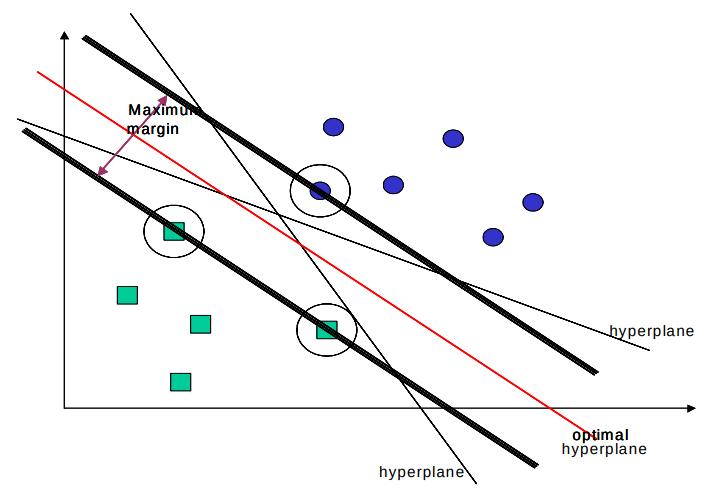
\includegraphics[width=1\textwidth]{SVM_max_margin}
	\caption{Maximálne rozpätie\cite{prop:SupervisedMachineLearning}}
	\label{pic:SVMMAxMargin}
\end{figure}

Avšak väčsina reálnych problémov zahŕňa nelineárne rozdelenie dát pre ktoré neexistuje žiadna hyper--rovina ktorá by úspešne rozdelila trénovacie dáta.
Riešenie tohto problému je mapovať dáta do vyššie--dimenzionálneho priestoru a definovať rozdeľujúcu hyper--rovinu tam.
Tento vyššíe-dimenzionálny priestor je nazývaný transformovaný priestor príznakov[eng. transformed feature space], ako opak ku vstupnému priestoru[eng. input space] obsahujúci trénovacie dáta\cite{prop:SupervisedMachineLearning}.

Pri vhodne zvolenom transformovanom priestore príznakov dostatočnej veľkosti, môžu byť každé treningové dáta rozdelitelné.
Lineárne rozdelenie v transformovanom priestore príznakov zodpovedá nelineárnemu rozdeleniu v pôvodnom vstupnej priestore.

Mapovanie dát do nejakého iného Hilbertovho priestora \cite{prop:HilbertSpace} $H$ ako $\Phi:R^d \rightarrow H$.
Potom trénovací algoritmus záležal len na údajoch zo skalárneho súčinu[eng. dot products] v priestore $H$, t.j na funkciách v tvare $\Phi(x_i) * \Phi(x_j)$.


%- obrazok pre scikit-learn.org/stable/modules/svm.html\#classification

\subsection{Stochastic Gradient Descent}

\subsection{Neural Network}
- 17150\_FULLTEXT.pdf - Background str.25, Deep learning str.30

- DiplomovaPraca.pdf - HLBOKÉ UČENIE A NEURÓNOVÉ SIETE str.20

- DP\_MajtánMartin.pdf - 1 NEURÓNOVÉ\ SIETE str.10

- FIT\_neuronky.pdf - Kap 3 Neuronové siete str.21

O čom je všeobecne Maching Learning
[Useful-things-about-machine-learning]

Machine Learning sa pouziva v širokej škále oblasti npr .....
My sme sa rozhodli použit ho na detekovanie typu zbrane a náklonu zbrane v obrazovej scéne.


%\subsection{Decision Trees}
%Asi NIE
%http://scikit-learn.org/stable/modules/tree.html


- Mozno dat Deep Learning in computer vision z 17150\_FULLTEXT.pdf, ako bouncing box a pod...
Nech tu mam nieco na detekciu a nie len klasifikacia.

\section{Predspracovanie obrazu}
http://scikit-image.org/docs/dev/auto\_examples/

\subsection{Hogova transformacia}
- F3-DP-2016-Erlebach-Jonas-Automaticka detekce pupily v obraze.pdf

\subsection{Detekcia hran}

- Sobelov filter - podľa knižky patri medzi najpopulárnejšie hranové filter.
Urobiť z neho magnitúdu obrazu potom.

% ------------ NEW CHAPTER ------------
\chapter{Návrh riešenia}

- Exploiting-the-complementary-strengths-of-multi-layer-CNN-image-retrieval.pdf,
preco pouzivat CNN na tento problem

\section{Keras}
- 17150\_FULLTEXT.pdf - Tensorflow and Keras str.26

- Navrhovana technologia pre ucenie

\section{scikit-learn}
- Kratky popis

\section{Databáza zbraní}
- ....

\section{Klasifikácia typu zbrane}

\section{Určenie natočenia zbrane}


% ------------ NEW CHAPTER ------------
\pagebreak
\chapter{Implementácia}

\section{Dataset}
